\documentclass{beamer}
\usepackage[utf8]{inputenc}
\usepackage{amsthm}
\usepackage{amsmath}
\usepackage{graphicx}
%\usetheme{Copenhagen}
\usetheme{Madrid}
%\usecolortheme{crane}
\setbeamercolor{titlelike}{parent=structure,bg=black,fg=white}
\setbeamercolor{subsection in head/foot}{bg=black,fg=white}
\setbeamercolor{frametitle}{bg=black}
\setbeamercolor*{palette primary}{bg=black!40!white, fg = white}
\setbeamercolor*{palette secondary}{bg=black!60!white, fg = white}
\setbeamercolor*{palette tertiary}{bg=black, fg = white}
\setbeamercolor*{palette quaternary}{bg=black!40!white, fg = white}





\title{Control System Problem}
\author{R. Sai Karthik}
\institute{IIT Hyderabad}

\begin{document}
\begin{frame}
\titlepage    
\end{frame}
\begin{frame}{Contents}
\tableofcontents
\end{frame}
\section{Question}
\begin{frame}{Question}
The asymptotic Bode phase plot of $\textbf{G(s)}=\frac{\textbf{k}}{\textbf{(s+0.1)}\textbf{(s+10)}\textbf{(s+p1)}}$, with \textit{k} and \textit{$p_1$} both positive, is shown below.
\[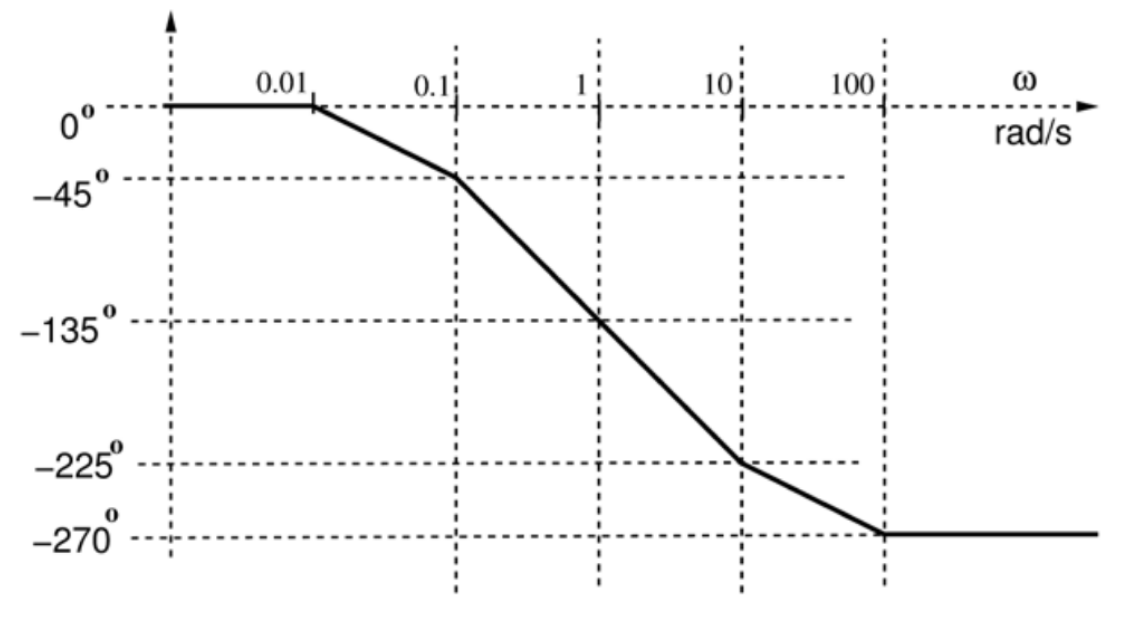
\includegraphics[scale = 0.2]{image.png}\]
Find the value of \textit{$p_1$}.
\end{frame}


\section{Theory Needed To Solve This Problem}
\begin{frame}{Theory Needed To Solve This Problem}
Phase plot of a transfer function is calculated by substituting s with j$\omega$.
\\
Since, the phase of a+ib is $\arctan(\frac{b}{a}$)
\\
for a transfer function having $z_1,z_1$ has zeroes and $p_1,p_2,p_3$ has poles,
\[phase = \arctan(\frac{\omega}{z_1})+\arctan(\frac{\omega}{z_2})-\arctan(\frac{\omega}{p_1})-\arctan(\frac{\omega}{p_2})-\arctan(\frac{\omega}{p_3}) \]

\end{frame}




\section{Solution}
\begin{frame}{Solution}
Phase of this transfer function
\\
\[\phi(\omega) = -\arctan(\frac{\omega}{0.1}) -\arctan(\frac{\omega}{10}) -\arctan(\frac{\omega}{p_1})\]
From the plot, at $\omega = 0.1$ $\phi$  $is -45^{\circ}$
\[ -45^{\circ} = -\arctan(\frac{0.1}{0.1}) -\arctan(\frac{0.1}{10}) -\arctan(\frac{0.1}{p_1})\]
\[ -45^{\circ} = -\arctan(1) -\arctan(\frac{1}{100}) -\arctan(\frac{1}{10p_1})\]
\[ -45^{\circ} \approx -\arctan(\frac{0.1}{0.1}) -\arctan(\frac{0.1}{10}) -\arctan(\frac{0.1}{p_1})\]

\end{frame}



\begin{frame}{Solution}
On Solving We get the $p_1$ is approximately 1, i.e, for $p_1$ in 0.95 to 1.05 the $\phi$ is approximately equals to $-45^{\circ}$.

Another way by intution, We know that in asymptotic Bode plot for a single pole has $-45^{\circ}$ at the pole and changes from 0 to -90 in 10 decades i.e, from $p/10$ to 10p
  
\end{frame}


\begin{frame}{Solution}
So by adding the bodeplots corresponding to the 0.1,10 and $p_1$ poles we get the required bodeplot.
By observing the bodeplots corresponding to 0.1 and 10,
\[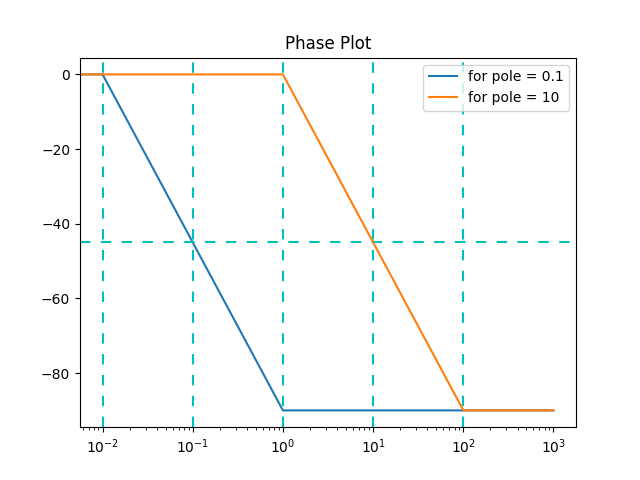
\includegraphics[scale = 0.5]{image3.png}\]
\end{frame}
\begin{frame}{Solution}
The values before the 0.1 does not change when compared to the given plot, so $p_1/10$ is greater than or equal to 0.1.
In the plot obtained by adding these two plots the slope at 0.1 doesnt change, but in the given plot there is a change so $p/10 = 0.1 $ 
\
$\implies p_1 = 1$
\end{frame}

\begin{frame}
\[\textbf{THANK \ YOU!}\]
\end{frame}

\end{document}